% THIS IS SIGPROC-SP.TEX - VERSION 3.1
% WORKS WITH V3.2SP OF ACM_PROC_ARTICLE-SP.CLS
% APRIL 2009
%
% It is an example file showing how to use the 'acm_proc_article-sp.cls' V3.2SP
% LaTeX2e document class file for Conference Proceedings submissions.
% ----------------------------------------------------------------------------------------------------------------
% This .tex file (and associated .cls V3.2SP) *DOES NOT* produce:
%       1) The Permission Statement
%       2) The Conference (location) Info information
%       3) The Copyright Line with ACM data
%       4) Page numbering
% ---------------------------------------------------------------------------------------------------------------
% It is an example which *does* use the .bib file (from which the .bbl file
% is produced).
% REMEMBER HOWEVER: After having produced the .bbl file,
% and prior to final submission,
% you need to 'insert'  your .bbl file into your source .tex file so as to provide
% ONE 'self-contained' source file.
%
% Questions regarding SIGS should be sent to
% Adrienne Griscti ---> griscti@acm.org
%
% Questions/suggestions regarding the guidelines, .tex and .cls files, etc. to
% Gerald Murray ---> murray@hq.acm.org
%
% For tracking purposes - this is V3.1SP - APRIL 2009

\documentclass{edm_template}

% Load basic packages
\usepackage{balance}  % to better equalize the last page
\usepackage{graphics} % for EPS, load graphicx instead 
\usepackage[T1]{fontenc}
\usepackage{txfonts}
\usepackage{mathptmx}
\usepackage[pdftex]{hyperref}
\usepackage{color}
\usepackage{booktabs}
\usepackage{textcomp}
\usepackage{booktabs}
% Some optional stuff you might like/need.
\usepackage{microtype} % Improved Tracking and Kerning
% \usepackage[all]{hypcap}  % Fixes bug in hyperref caption linking
\usepackage{ccicons}  % Cite your images correctly!
% \usepackage[utf8]{inputenc} % for a UTF8 editor only

%\usepackage{algorithm} 
\usepackage[ruled]{algorithm}
\usepackage{algpseudocode}
\usepackage{algorithmicx} 

% If you want to use todo notes, marginpars etc. during creation of your draft document, you
% have to enable the "chi_draft" option for the document class. To do this, change the very first
% line to: "\documentclass[chi_draft]{sigchi}". You can then place todo notes by using the "\todo{...}"
% command. Make sure to disable the draft option again before submitting your final document.
\usepackage{todonotes}

\usepackage{amssymb}
\usepackage{amsmath,scalerel}

\usepackage{graphicx}
\usepackage{epstopdf}
%\usepackage{natbib}
\usepackage{array}
\usepackage{color} 
\newcommand{\hl}[1]{\colorbox{yellow}{#1}}
\usepackage{subcaption}
\usepackage{enumitem}
\usepackage{url}

\DeclareMathOperator*{\argmax}{arg\,max}
\DeclareMathOperator*{\Bigcdot}{\scalerel*{\cdot}{\bigodot}}

\usepackage{tikz}
\usetikzlibrary{decorations.pathreplacing,calc}
\newcommand{\tikzmark}[1]{\tikz[overlay,remember picture] \node (#1) {};}
\newcommand*{\AddNote}[4]{%
	\begin{tikzpicture}[overlay, remember picture]
	\draw [decoration={brace,amplitude=0.2em},decorate, thick, darkgray]
	($(#3)!(#1.north)!($(#3)-(0,1)$)$) --  
	($(#3)!(#2.south)!($(#3)-(0,1)$)$)
	node [align=center, text width=2.5cm, pos=0.5, anchor=west] {#4};
	\end{tikzpicture}
}%
\usepackage{tabularx}
\usepackage{multirow}


\algdef{SE}[DOWHILE]{Do}{doWhile}{\algorithmicdo}[1]{\algorithmicwhile\ #1}%

\begin{document}
	
	\title{Towards Automatic Discovery of Prerequisite Structure of Skills from Student Performance Data}
	%\subtitle{[Extended Abstract]
	%\titlenote{A full version of this paper is available as
	%\textit{Author's Guide to Preparing ACM SIG Proceedings Using
	%\LaTeX$2_\epsilon$\ and BibTeX} at
	%\texttt{www.acm.org/eaddress.htm}}}
	%
	% You need the command \numberofauthors to handle the 'placement
	% and alignment' of the authors beneath the title.
	%
	% For aesthetic reasons, we recommend 'three authors at a time'
	% i.e. three 'name/affiliation blocks' be placed beneath the title.
	%
	% NOTE: You are NOT restricted in how many 'rows' of
	% "name/affiliations" may appear. We just ask that you restrict
	% the number of 'columns' to three.
	%
	% Because of the available 'opening page real-estate'
	% we ask you to refrain from putting more than six authors
	% (two rows with three columns) beneath the article title.
	% More than six makes the first-page appear very cluttered indeed.
	%
	% Use the \alignauthor commands to handle the names
	% and affiliations for an 'aesthetic maximum' of six authors.
	% Add names, affiliations, addresses for
	% the seventh etc. author(s) as the argument for the
	% \additionalauthors command.
	% These 'additional authors' will be output/set for you
	% without further effort on your part as the last section in
	% the body of your article BEFORE References or any Appendices.
	
	\numberofauthors{3} %  in this sample file, there are a *total*
	% of EIGHT authors. SIX appear on the 'first-page' (for formatting
	% reasons) and the remaining two appear in the \additionalauthors section.
	%
	\author{%
		\alignauthor{Leave Authors Anonymous\\
			\affaddr{for Submission}\\
			\affaddr{City, Country}\\
			\email{e-mail address}}\\
		\alignauthor{Leave Authors Anonymous\\
			\affaddr{for Submission}\\
			\affaddr{City, Country}\\
			\email{e-mail address}}\\
		\alignauthor{Leave Authors Anonymous\\
			\affaddr{for Submission}\\
			\affaddr{City, Country}\\
			\email{e-mail address}}\\	
	}
	
\maketitle
\begin{abstract}
Knowing the prerequisite structure of skills is crucial for designing curriculum, assessing mastery and for student modeling.
These prerequisite structures are hand-engineered by subject matter expert in a costly and time-consuming process.
%Traditionally, the prerequisite structures of skills are manually specified by human experts and this process is often time-consuming.
%Automatic discovery of the prerequisite structures from educational data is intriguing yet challenging since student's mastery of skills are latent variables.
In this paper, we introduce a novel data-driven pipeline for inferring the prerequisite structure of skill from student performance on test items. 
By modeling the prerequisite relations as a Bayesian network, the pipeline estimates the causal structure and the probabilistic dependence among the skills 
via a two-stage learning process. 
In the first stage, the Structural Expectation Maximization (Structural EM) algorithm is used to select a class of Bayesian networks based on distribution fitting of student data;
in the second stage, a single Bayesian network structure is determined by enforcing a constraint on the estimated conditional probability tables.
We validate the proposed pipeline using simulations and by post-hoc analysis of student data.
We show the discovered prerequisite structures can improve the student model in predicting student performance. 
\end{abstract}

%% A category with the (minimum) three required fields
%\category{H.4}{Information Systems Applications}{Miscellaneous}
%%A category including the fourth, optional field follows...
%\category{D.2.8}{Software Engineering}{Metrics}[complexity measures, performance measures]
%
%\terms{Theory}

\keywords{ACM proceedings, \LaTeX, text tagging} % NOT required for Proceedings

\section{Introduction}
\label{sec:introduction}
%Students usually acquire knowledge components in a meaningful sequence which starts from relatively simple concepts and gradually approaches more complex ones. 
Students learn much better when the skills are not randomly introduced 
but organized in a meaningful order which starts from relatively simple concepts and gradually introduces more complex ones. 
Further, among these skills, some are preliminary of others such that they must be mastered before the subsequent concepts can be learned.
For instance, students have to know how to do addition before they learn to do multiplication.
In this work, we use prerequisite structure to refer to the relationships among skills that place strict constraints
on the order in which these skills can be acquired. Determining the prerequisite relations among skills is crucial for designing curriculum and for assessing mastery.

Most prerequisite structures of skills are hand-engineered by subject matter experts in a costly and time-consuming process. 
Further, the prerequisite structures specified by the experts are seldom tested and might be unreliable in
the sense that experts may hold ``blind spots".
Nowadays, large volume of educational data has been cumulated through the online tutoring systems.  
Thus, learning prerequisite structures from educational data has drawn substantial interest from both education and data mining communities \cite{desmarais2006learned,vuong2010method, brunskill2010estimating,scheines2014discovering,chen2015discovering,piech2015deep}.
However, inferring the prerequisite relationships between skills is still challenging since a student's knowledge of a skill is a latent variable in the data.
In this paper, we introduce BNPD, a novel pipeline for discovering prerequisite structure of skills from data. 
BNPD models the prerequisite structure of the skills with a statistical model called Bayesian network.
It then learns the Bayesian network through a two-stage process. 


%In education, remedial interventions attempt to eliminate the specific effect of lacking a competency.
%Traditional and mastery-based educational strategies~\cite{bloom1968learning} often rely on remedial interventions when a learner is having a difficulty in the curriculum.
%Teachers often use their experience, knowledge and common sense to justify if a student may need remedial assistance.
%With the growing popularity of Intelligent Tutoring Systems, computers are starting  to have capabilities to detect when a student is in need of remediation.
%The process of designing when a computer should offer remediation to a student typically starts by subject matter experts writing rules that are then engineered into the system.
%These rules are difficult and time consuming to build.


%In this paper we introduce the \textit{Remedial Intervention Detector} (REMIND) algorithm.
%REMIND is a novel pipeline that uses data--and optionally domain knowledge-- to infer when a student may lack the  necessary  knowledge to solve the current lesson.
%We believe the capability of combining data with subject matter expertise is a promising approach.


%\section{Remedial Intervention Detector (REMIND) }
%In many instructional settings, students are graded by their performance on instruments such as exams or homework assignments. 
%Usually, these instruments are made of items--questions, problems, parts of questions-- which are graded individually.
%Modern applications of statistics in education often rely on a mapping of items to skills (often called a $Q$-matrix) to analyze data collected from students answering items.
%The item to skill mapping is often designed by subject matter experts, but automatic approaches exist~\cite{jp_aistats_2015}.
%
%REMIND is a pipeline that uses data from students answering items to discover when a student  is lacking background knowledge and could benefit from remediation.
%For this, REMIND first discovers prerequisite structures  among the skills in the data.
%In the context of this paper, we define the prerequisite structure as the strict constraints on the order in which these skills can be acquired.
%REMIND then uses student modeling techniques to infer if a student has mastered the skill and its prerequisites.
%The rationale is  that a student should receive a remedial intervention if she is likely to lack a prerequisite.%, an intervention for tutoring remedial content should be offered to the student.
%In \S~\ref{sec:learning_remind} we describe how to learn a REMIND  model from data;
%and in \S~\ref{sec:using_remind} we explain how to use it to offer remedial interventions.


\section{Previous Work}
\label{sec:previous_work}
Many works have investigated the discovery of prerequisite structures within domain models from data.
Some of these works aim to learn the prerequisite structure of observed variables, e.g., the relationships among exercise problems.
These include the Partial Order Knowledge Structures (POKS) algorithm \cite{desmarais2006learned, pavlik2008using} to learn the item-item relationships
and the approach to determine the dependency structure of units in a curriculum with the student performance data observed at the unit level \cite{vuong2011method}.
  
To learn the relationships among skills from data where a student's knowledge of a skill is latent, 
Brunskill proposed a method of computing and comparing the log likelihoods between the prerequisite model and the flat model (skills are independent) 
on each skill pair to determine which model better fits the data \cite{brunskill2010estimating}. 
Chen et al. \cite{chen2015discovering} then used probabilistic association rules mining to determine the prerequisite relationships between each pair of skills.
Both methods focus on estimating the pairwise prerequisite relationships, instead of optimizing the full structure of the skills.
%Moreover, these approaches require many preconditions. For example, Brunskill's method assumes domain parameters called \emph{guess probability} and \emph{slip probability} are provided for each pair of item and skill.
%Chen et al's approach requires manually specified thresholds to determine the existence of a prerequisite relationship.
%The determination of these thresholds requires experts' intervention. 

Bayesian networks have been extensively used to model skill topologies \cite{kaser2014beyond}.
By modeling prerequisite relations as a Bayesian network, Scheines et al. used a Bayesian network structural learning algorithm to find the Bayesian network structure that best represents the distribution of the data \cite{scheines2014discovering}.
Bayesian network allows encoding conditional independence relationships between skills, which enables more accurate modeling of the probabilistic dependence between skills.
However, output from their algorithm is a class of Bayesian networks. These Bayesian networks represent different prerequisite structures.

In this paper, we propose a novel pipeline to infer the prerequisite structures of skills. Our approach also uses Bayesian network to model the prerequisite relationships.
The pipeline first use a popular Bayesian network structure learning algorithm, 
called Structural EM to select a class of Bayesian network models based on the distribution fitting to the data.
It then uses constraint on the conditional probability tables to select one Bayesian network, which gives a unique prerequisite structure of skills.
Finally, we show the discovered prerequisite structure can be used to improve student modeling.

\section{The Prerequisite Structure Discovery Pipeline}
\label{sec:pre_pipeline}
BNPD learns the prerequisite structure of the skills using data with a statistical model called Bayesian network \cite{pearl2000causality,spirtes2001causation}.
Bayesian networks are also called probabilistic graphical models  because they can  be represented visually and algebraically as a collection of nodes and edges.
A tutorial description of Bayesian networks in education can be found elsewhere \cite{almond2015bayesian}, 
but for now we say that they are often described with two components: 
the  nodes represent the random variables, which we describe using \textit{conditional probability tables} (CPTs),
and the set of edges that form a \textit{directed acyclic graph} (DAG) represent the conditional dependencies between the variables.
Bayesian networks are a flexible tool that can be used to model an entire curriculum.

Figure~\ref{fig:smexample} illustrates an example of a prerequisite structure modeled with a Bayesian network.
Here, we relate four test items with the skills of addition and multiplication.
Addition is a prerequisite of multiplication thus there is an arrow from addition to multiplication.
Modeling prerequisites as edges in a Bayesian network allows us to frame the discovery of the prerequisite relationships as the well-studied machine learning problem of learning a DAG (with the presence of latent variables).


\begin{figure}
	\begin{center}
		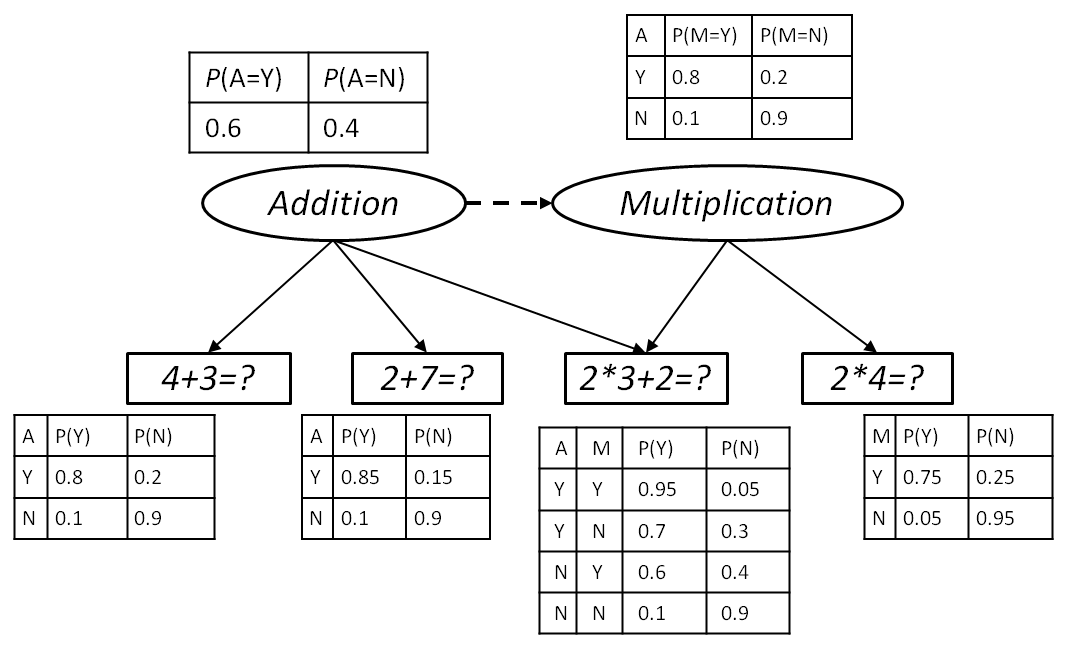
\includegraphics[width=1.0\linewidth]{figures/studentmodel.png}
	\end{center}
	\caption{A hypothetical Bayesian network learned with Algorithm~\ref{alg:remind}. 
		Solid edges are given by the item to skill mapping, dashed edges between skill variables are to be discovered from data.
		The conditional probability tables are to be learned.}
	\label{fig:smexample} 
\end{figure} 


Algorithm~\ref{alg:bnpd} describes the BNPD pipeline.
Suppose we collect data from  $n$ students, answering $p$ items.
Then, the input of BNPD is a matrix $\mathbf{D}$ with $n \times p$ dimensions, an item to skill mapping.%, and (optionally) some constraints on what content can trigger a remediation.
Each entry in $\mathbf{D}$ encodes the performance of a student (see Table~\ref{tbl:d-matrix} for an example).
%BNPD first constructs the prerequisite relationships among the set of skills using constraints.
%Then, it  learns the parameters of a student model  that infers what skills a student has mastered.


\begin{table}[htb]%\small
	\centering
	\caption{Example data matrix to use with BNPD.  The performance of a student is encoded with 1 if the student answered correctly the item, and 0 otherwise. \label{tbl:d-matrix}}
	\begin{tabular}{@{}lllll@{}}
		\toprule
		User  & Item 1 & Item 2 & Item 3 & Item $p$ \\ \midrule
		Alice & 0      & 1      &        & 0        \\
		Bob   & 1      & 1      & ...    & 1        \\
		Carol & 0      & 0      &        & 1        \\
		\multicolumn{5}{c}{...}                     \\ \bottomrule
	\end{tabular}
\end{table}


BNPD relies on a popular machine learning algorithm called Structural Expectation Maximization (EM), which has not been used in educational applications. 
A secondary contribution of our work is introducing Structural EM for learning Bayesian network structures from educational data.
%In particular, we modify Structural EM to be used for discovering the prerequisite relationships among skills from students' responses on test items.
%One of the advantages of Structural EM algorithm over prior work is that it allows to combine expert beliefs into the inference process.
%\hl{Say some advantages of Structural E-M, such that it allows expert beliefs to be engineered,  this helps so a remediation won't be content from the future, but only for the past, for example}
We now describe the  steps of BNPD in detail.

\begin{algorithm}
	\begin{algorithmic}[1]
		\Require A matrix $\mathbf{D}$ of student performance on a set of test items, skill-to-item mapping $Q$ (containing a set of skills $\mathbf{S}$).
		%and a set of constraints $\mathbf{C}$ reflecting experts' beliefs on the prerequisite structure
		\State  $G_0\leftarrow$ Initialize$(\mathbf{S}, Q)$ ~~~~~~~~~~~~~~~~\tikzmark{inittop}\tikzmark{right}
		\State $i\leftarrow 0$ \tikzmark{initbot}
		\Do \tikzmark{semtop}
		\State \emph{E}-step: 
		\State ~~~ $\theta_i^*\leftarrow$ ParametricEM($G_i,\mathbf{D}$) 
		\State ~~~ $\mathbf{D}_i^*\leftarrow$ Inference($G_i,\theta_i^*,\mathbf{D}$) 
		\State \emph{M}-step:
		\State ~~~ $\langle G_{i+1}, \theta_{i+1}\rangle\leftarrow$ BNLearning($G_i$,$\mathbf{D}_i^*$)
		\State ~~~ $i\leftarrow i+1$
		\doWhile{Stop criteria is not met}~~~~~~~~~~~~~~~~~~\tikzmark{right}\tikzmark{sembot}
		\State $RE\leftarrow FindReversibleEdges(G_i)$  ~~~~~~~~~~~~~~~~~\tikzmark{lsmtop}\tikzmark{right}
		\State $EC\leftarrow EnumEquivalentDAGs(G_i)$
		\State $DE\leftarrow \{\}$
		\For{every reversible edge $S_i - S_j$ in $RE$}
		%\State Compute $P(S_i=1|S_j=1)$, $P(S_j=0|S_i=0)$\\~~~~~$P(S_j=1|S_i=1)$ and $P(S_i=0|S_j=0)$
		\State $ratio\leftarrow\frac{P(S_i=1|S_j=1)\cdot P(S_j=0|S_i=0)}{P(S_j=1|S_i=1)\cdot P(S_i=0|S_j=0)}$\footnote{}
		\If {$ratio>1$}
		\State $ratio^*=ratio$
		\State $DE\leftarrow DE\cup S_i\rightarrow S_j$ 
		\Else
		\State $ratio^*=\frac{1}{ratio}$
		\State $DE\leftarrow DE\cup S_i\leftarrow S_j$
		\EndIf
		\EndFor
		\State $sort(DE)$ by $ratio^*$ in descending order
		\While{$DE$ is not empty}
		\State $e\leftarrow dequeue(DE)$
		\State $\forall G\in EC$, remove $G$ from $EC$ if $e\notin G$
		\EndWhile
		\State return $EC$ 		
		\tikzmark{lsmbot}
	\end{algorithmic}
	\AddNote{inittop}{initbot}{right}{\footnotesize Initialization}
	\AddNote{semtop}{sembot}{right}{\footnotesize Structural EM}
	\AddNote{lsmtop}{lsmbot}{right}{\footnotesize Orient edges}
	\caption{The BNPD algorithm\label{alg:bnpd}}
\end{algorithm}
\footnotetext{$P(S_i=a|S_j=b)$ can be computed using any Bayesian network inference algorithm such as Junction tree algorithm\cite{koller2009probabilistic}}

\subsection{Initial Bayesian Network}

BNPD represents the prerequisite structure using Bayesian networks that use latent variables to represent the student knowledge of a skill, 
and observed variables that represent the student performance answering items (e.g, correct or incorrect).
We first create an initial Bayesian network that complies to the skill-to-item $Q$-matrix
% and a set of constraints reflecting experts' belief
on the prerequisite structure 
%(step 1 of Algorithm~\ref{alg:remind}).
That is, we create an arc to each item from each of its required skills and leave all skill variables disconnected.
With the created Bayesian network as an initial network, we learn the arcs between the skill variables using Structural EM.

\subsection{Structural EM}

A common solution to learning a Bayesian network from data is the score-and-search approach \cite{cooper1992bayesian,heckerman1997bayesian}.
This approach uses a scoring function\footnote{A commonly used scoring function is Bayesian information criterion (BIC), which is composed of a likelihood term and a term to penalize the model complexity} to measure the fitness of a Bayesian network structure to the observed data, 
and manages to find the optimal model in the space of all possible Bayesian network structures.
However, the conventional score-and-search approaches rely on efficient computation of the scoring function, 
which is only feasible for problems where data contains observations for all variables in the Bayesian network.
Unfortunately, our domain has skill variables that are not directly observed.
An intuitive work-around is to use the Expectation Maximization (EM) to estimate the scoring function.
However, EM in this case takes a large number (hundreds) of iterations to converge and each iteration requires Bayesian network inference, 
which is computationally prohibitive.
Further, we need run EM for each candidate structure. The number of possible Bayesian network structures is super-exponential with respect to the number of nodes.
The Structural Expectation Maximization algorithm \cite{friedman1997learning,friedman1998bayesian} is an efficient alternative.
%We now summarize how it works.

Structural EM is an iterative algorithm that  inputs a matrix $\mathbf{D}$ of student performance (see example Table~\ref{tbl:d-matrix}). %, where columns are the set of exercise items $\mathbf{I}$ and each row contains a student's performances on all these exercise items.
Figure~\ref{fig:sem} illustrates one iteration of the Structural EM algorithm. The relevant steps are also sketched in Algorithm~\ref{alg:bnpd}. 
Each iteration consists of an Expectation step (\emph{E-step}) and a Maximization step (\emph{M-step}). 
%Structural EM calculates in each iteration a candidate model structure $G$ be by iterating over the Expectation and Maximization steps.
In \emph{E-step}, we first find the maximum likelihood estimate $\theta^*$ of the parameters 
for the current structure $G$ calculated from previous iteration using parametric EM.\footnote{In the first iteration, the current network is created from the initialization step.}
We then do Bayesian inference to compute the expected values for the hidden variables using the current model $(G,\theta^*)$
and use the values to complete the data.
In the \emph{M-step}, we use the conventional score-and-search approach to optimize the structure according to the completed data.
Since the space of possible Bayesian network structures is super-exponential, 
exhaustive search is intractable and local search algorithms, such as greedy hill-climbing search, are often used.
The \emph{E-step} and \emph{M-step} interleave and iterate until some stop criteria is met, e.g., the scoring function does not change significantly.
Contrast to the conventional score-and-search algorithm, Structural EM runs EM only on one structure in each iteration, thus is computationally more efficient.

\begin{figure}
	\begin{center}
		%\framebox[4.0in]{$\;$}
		%\fbox{\rule[-.5cm]{0cm}{4cm} \rule[-.5cm]{4cm}{0cm}}
		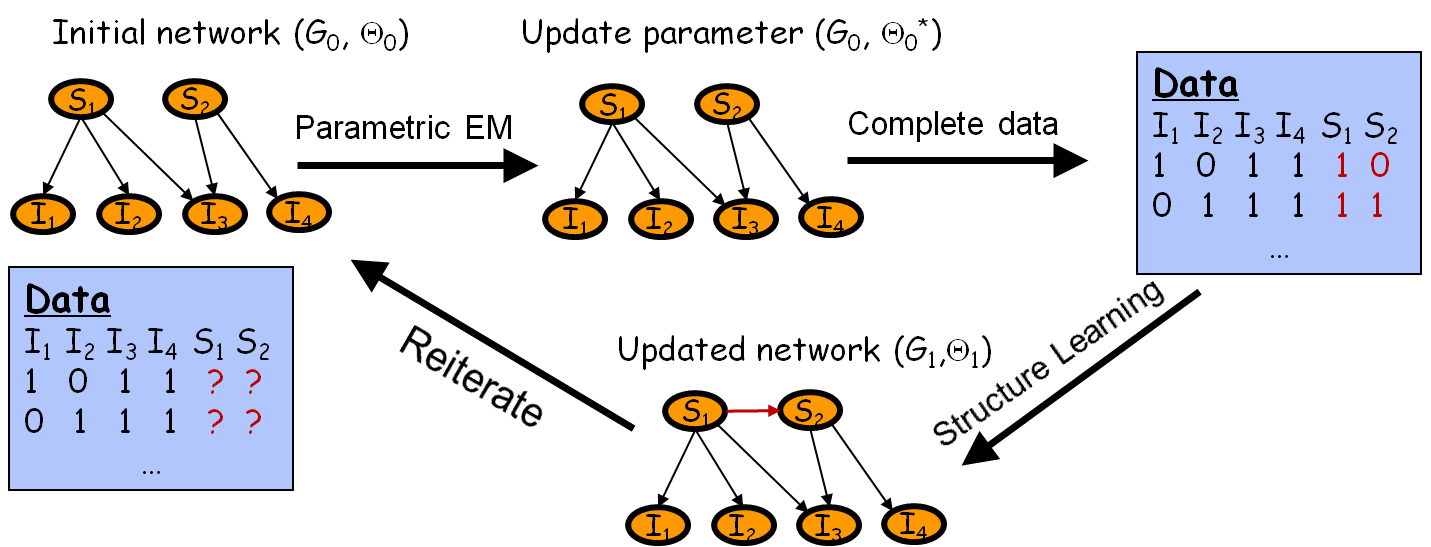
\includegraphics[width=1.0\linewidth]{figures/sem.png}
	\end{center}
	\caption{\small An illustration of the Structure EM algorithm to discover the structure of the latent variables.}
	\label{fig:sem} 
\end{figure} 

BNPD's  initialization step
%REMIND's implementation of prerequisite discovery we use Structural EM to learn the arcs between skills, but 
fixes the arcs from skills to items according to the ${Q}$-matrix.
%For this, we initialize the network as $G_0$ where skill variables and item variables are connected according to the ${Q}$-matrix, but skill variables are disconnected with each other. 
In  the \emph{M-step} of our Structural EM implementation we only consider the candidate structures that comply with the ${Q}$-matrix.
%We believe that this reduction of the space of candidate models improves efficiency. %makes the Structural EM more efficient.

An advantage of using Structural EM to discover the prerequisite relationship of skills, is that it is easily extensible to incorporate domain knowledge.
For example, we can  place constraints on the output structure to force or to disallow a skill to be a prerequisite from another other skill.
Consider,  an intelligent tutor that teaches the content of a book. 
The book content structure provides a natural ordering of the chapters. 
We may use the book structure to engineer domain knowledge that an introductory chapter cannot be prerequisite of content that appears later in the book.

Another advantage of Structural EM is that it can be applied when there are missing data in the student performance matrix $\mathbf{D}$. 
That is, some students do not answer all the items thus some responses are missing. This ``missing values" problem is very common in real-world situations.
Structural EM can be applied to this type of data since it was originally developed to solve the "missing values" problem \cite{friedman1997learning}.
The general idea is, in the \emph{E-step}, the algorithm also computes the expected values for missing data points, in addition for hidden variables, . 

\subsection{Discriminate Between Equivalent BNs}

Structural EM selects Bayesian network model based on how well it explains the distribution of the data. 
Bayesian network theory states that some Bayesian networks are statistically equivalent in representing the data.
Thus, the output from Structure EM is an equivalence class that may contain many Bayesian network structures.
These equivalent Bayesian networks have the same skeleton and the same $v$-structures\footnote{
A $v$-structure in a Bayesian network $G$ is an ordered triple of nodes $(u,v,w)$ such that $G$ contains the directed edges $u\rightarrow v$ and $w\rightarrow v$ and $u$ and $w$ are not adjacent in $G$. \cite{verma1990equivalence}.}. 
For instance, Figure~\ref{fig:equivnets} gives an example of three simple Bayesian networks that are not distinguishable by Structural EM algorithm.
They share the skeleton but differ in the orientation of the edge. They apparently represent three different prerequisite structures.
To determine which structure is the case, we shall determine the orientation of each reversible edge.
For this purpose, we can use the following domain knowledge.

\textbf{Knowledge 1}. If $S_1$ is a prerequisite of $S_2$, i.e., $S_1\rightarrow S_2$, then $P(S_1=1|S_2=1)= 1$ and $P(S_2=0|S_1=0)= 1$.

\textbf{Knowledge 1} says if a skill $S_1$ is the prerequisite of a skill $S_2$,
a student must master skill $S_1$ before he masters $S_2$ and it is impossible for him to master $S_2$ if he has not mastered $S_1$.
In other words, $S_1$ is not a prerequisite of $S_2$ if at least one of the conditions does not hold.
This puts a constraint on the joint distribution encoded by the Bayesian network to be learned.
We can check for each reversible edge $S_i-S_j$ in the Bayesian network, either $P(S_i=1|S_j=1)= 1$ and $P(S_j=0|S_i=0)= 1$, or $P(S_j=1|S_i=1)= 1$ and $P(S_j=0|S_i=0)= 1$. 
If the former holds, $S_i\rightarrow S_j$; otherwise, $S_i\leftarrow S_j$.  
However, in real situations, it is possible for a student to master the post-requisite even he does not know the prerequisite. 
Further, there is always noise in the data. Thus, the two conditional probabilities $P(S_1=1|S_2=1)$ and $P(S_2=0|S_1=0)$ are not exactly but close to 1.
Thus, we use the following empirical rule: if $P(S_1=1|S_2=1)\cdot P(S_2=0|S_1=0)>P(S_2=1|S_1=1)\cdot P(S_1=0|S_2=0)$, we determine $S_1\rightarrow S_2$; 
otherwise, we determine $S_1\leftarrow S_2$. 
The intuition behind this is that the two probabilities $P(S_1=1|S_2=1)$ and $P(S_2=0|S_1=0)$ are certificates of the prerequisite structure $S_1\rightarrow S_2$.
The larger of these two probabilities, the more likely the relationship $S_1\rightarrow S_2$ holds.
Since here we are concerned with which direction the edge goes, we simply compare the products of two probabilities and select the direction that is more probable. 

	\begin{figure}[!ht]\small
		\centering
		\begin{subfigure}[t]{0.32\linewidth}
			\centering
			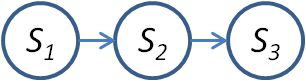
\includegraphics[width=0.9\linewidth]{figures/s1s2s3.png}
			\caption{\label{fig:equivnet1}}
			%$P(S_1=1|S_2=1)=0.86$ \\ $P(S_2=0|S_1=0)=0.92$
		\end{subfigure}
		\begin{subfigure}[t]{0.32\linewidth}
			\centering
			
\includegraphics[width=0.9\linewidth]{figures/s2s1s3.png}
			\caption{\label{fig:equivnet2}}
			%$P(S_2=1|S_1=1)=0.52$ \\ $P(S_1=0|S_2=0)=0.64$
		\end{subfigure}
		\begin{subfigure}[t]{0.32\linewidth}
			\centering
			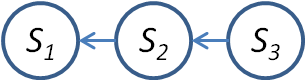
\includegraphics[width=0.9\linewidth]{figures/s3s2s1.png}
			\caption{\label{fig:equivnet3}}
			%$P(S_2=1|S_1=1)=0.52$ \\ $P(S_1=0|S_2=0)=0.64$
		\end{subfigure}		
		\caption{Three equivalent Bayesian networks representing different prerequisite structures.\label{fig:equivnets} }
	\end{figure}

Using the empirical rule, we can orient every reversible edge in the network structure. 
However, determining orientations for all reversible edges are not independent and may conflict each other.
Having oriented one edge would constrain the orientation of other reversible edges because we have to ensure the graph is a DAG and the equivalence is not violated.
For example, in Figure~\ref{fig:equivnet1}, if we have determined $S_1\rightarrow S_2$, the edge $S_2\rightarrow S_3$ is enforced.
In this paper, we take an ad-hoc strategy to determine the orientation for all reversible edges. 
For each reversible edge $S_i-S_j$, we compute $ratio=\frac{P(S_i=1|S_j=1)\cdot P(S_j=0|S_i=0)}{P(S_j=1|S_i=1)\cdot P(S_i=0|S_j=0)}$,
then  $ratio^*=ratio$ if $ratio >1$ and $ratio^*=\frac{1}{ratio}$ otherwise. The larger the $ratio^*$ is, the more confidently when we decide the orientation.
We sort the list of reversible edges by $ratio^*$ in descending order. We then orient the edges in this order.
When one edge is oriented, the constraint is propagated to other reversible edges. In practical implementation, we take a different strategy: 
we first enumerate all equivalent Bayesian networks and make them a list of candidates; 
when an edge is oriented to $S_i\rightarrow S_j$, we remove all contradicting Bayesian networks from the list.
Eventually only one Bayesian network structure stands. This procedure is also detailed in the \emph{Orient edges} section of Algorithm~\ref{alg:bnpd}.  
The $EnumEquivalentDAGs(G_i)$ implements the algorithm of enumerating equivalent DAGs proposed in \cite{chen2014finding}.

\section{Evaluation}
In \S~{\ref{sec:synthetic}, we  evaluate BNPD with simulated data  to assess the quality of the discovered prerequisite structures.
Then, in \S~\ref{sec:real} we  use  data collected from real students.
In all our experiment, we use the Bayesian information criterion (BIC) as the scoring function in Structural EM . 
%The BIC score for a Bayesian network model is composed of a likelihood term and a term to penalize the model complexity.

	\subsection{Simulated Data}
	\label{sec:synthetic}
	%We first use synthetic data to demonstrate the capability of Structural EM in learning the prerequisite structure of latent skill variables.
	%By using 
	%various factors, including sample size, number of skill or item variables, prior knowledge, noises in the data, 
	%affect the learning performance.
	
	Synthetic data allows us to study how BNPD compares to ground truth.
	For this, we engineered three prerequisite structures (DAGs), shown in Figure~\ref{fig:syn-nets}.
	Here, each figure represents different causal relations between the simulated latent skill variables.
	%Note that some edges are reversible and represented as undirected edges. 
	%Given observational data, the direction of some edges cannot be determined because the edges are \emph{reversible}%
	%We represent these edges as undirected lines.
	
	\begin{figure}[!ht]
		%\begin{center}
		\begin{minipage}[b]{0.45\linewidth}
			\centering
			
\includegraphics[width=0.9\linewidth]{figures/model1.png}\\~\\
			(a) Structure 1~\\~\\~\\
			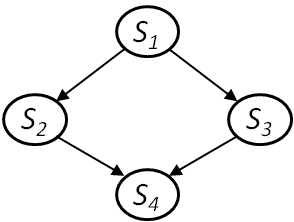
\includegraphics[width=0.8\linewidth]{figures/model2.png}\\~\\
			(b) Structure 2
		\end{minipage}
		\quad
		\begin{minipage}[b]{0.45\linewidth}
			\centering
			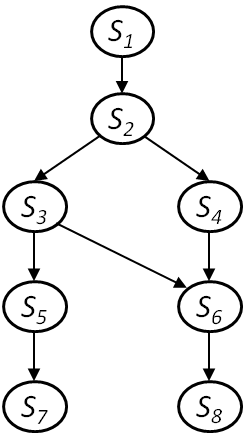
\includegraphics[width=0.7\linewidth]{figures/model3.png}\\~\\
			(c) Structure 3
		\end{minipage}	
		\caption{Three different DAGs between latent skill variables.  Item nodes are omitted.}
		\label{fig:syn-nets}
		%\end{center} 
	\end{figure} 
	
	For clarity, Figure~\ref{fig:syn-nets}  omits the item nodes;
	but each skill node is parent of six item variables and each item variable has 1-3 skill nodes as parents.
	All of these nodes are modeled using binary random variables.
	More precisely, the latent  nodes represent whether the student  achieves mastery of the skill,
	and the observed nodes indicate if the student answers the item correctly.
	Notice that these Bayesian networks include the prerequisite structures as well as the skill-item mapping.
	
	We consider simulated data with different number of observations ($n=150, 500, 1000, 2000$).
	For each sample size and each  DAG, we generate ten different sets of conditional probability tables
	%\footnote{10 random samples were generated for each sample size and each synthetic Bayesian network model.} %\todo{I reworded this paragraph, please check if it is correct}
	%We generate conditional probability tables
	randomly, with two  constraints.
	First, we enforce that achieving mastery of the prerequisites of a skill will increase the likelihood of mastering the skill.
	Second, mastery of a skill increases the probability of student correctly answering the test item. 
	Thus, in total we generated 120 synthetic datasets (3 DAGs x 4 sample sizes x 10 CPTs), and  report the average results.
	
	
	We evaluate how BNPD can discover the true prerequisite structure using metrics designed to evaluate Bayesian networks structure discovery.
	In particular, we use the $F_1$ \emph{adjacency score} and the $F_1$ \emph{orientation score}.
	The adjacency score measure how well we can recover connections between nodes.
	It is a weighted average of the true positive adjacency rate and the true discovery adjacency rate.
	On the other hand, the orientation score measures how well we can recover the direction of the edges.
	%To measure the accuracy of edge orientation, we compute the $F_1$ \emph{orientation score}, 
	It is calculated as a weighted average of the true positive orientation rate and true discovery orientation rate.
	%This metric does not account for the directionality incorrect edges that are reversible.
	In both cases, the $F_1$ score reaches its best value at 1 and worst at 0. 
	Moreover, for comparison, we compute the $F_1$ \emph{adjacency score} for Bayesian network structures whose skill nodes are fully connected with each other. 
	These fully connected DAGs will serve as baselines for evaluating the adjacency discovery.\footnote{We do not compute $F_1$ orientation score for fully connected DAGs because all edges in a fully connected DAG are reversible.}
	For completeness, we list these formulas in tables~\ref{tbl:ar}~and~\ref{tbl:or}, respectively.
	
	
	% Please add the following required packages to your document preamble:
	% \usepackage{booktabs}
	\begin{table}[ht]
		\centering
		\caption{Formulas for measuring adjacency rate (AR) \label{tbl:ar}}
		\label{my-label}
		\begin{tabular}{@{}ll@{}}
			\toprule
			Metric & Formula \\ \midrule
			True positive    (\emph{TPAR}) & $\frac{ \text{\# of correct adjacencies in learned model} } { \text{ \# of adjacencies in true model} }$  \\
			True discovery (\emph{TDAR}) &  $\frac{ \text{\# of correct adjacencies in learned model} } { \text{ \# of adjacencies in learned model} }$ \\
			$F_1$-\textit{AR} &  $\frac{2\cdot \text{\emph{TPAR}} \cdot \text{\emph{TDAR}}} {\text{\emph{TPAR}}+\text{\emph{TDAR}}}$  \\
			\bottomrule
		\end{tabular}
	\end{table}
	
	
	\begin{table}[th]
		\centering
		\caption{Formulas for measuring orientation rate (OR) \label{tbl:or}}
		\label{my-label}
		\begin{tabular}{@{}ll@{}}
			\toprule
			Metric & Formula \\ \midrule
			True positive  (\emph{TPOR}) & $\frac{ \text{\# of correctly directed edges in learned model} } {\text{ \# of directed edges in true model}}$  \\
			True discovery   (\emph{TDOR})& $\frac{ \text{\# of correctly directed edges in learned model } }{\text{ \# of directed edges in learned model}} $\\
			$F_1$-\textit{OR} &  $\frac{  2\cdot \text{\emph{TPOR}} \cdot \text{\emph{TDOR}} }{\text{\emph{TPOR}}+\text{\emph{TDOR}}}$ \\
			\bottomrule
		\end{tabular}
	\end{table}
	
	We use these metrics to evaluate the effect of varying the  number of observations  of the training set (sample size) on the quality of learning the prerequisite structure.
	We designed experiments to specifically answer the following four questions:
	\begin{enumerate}[noitemsep,topsep=2pt,parsep=0pt,partopsep=0pt]
		\item How does the type of items affect BNPD's ability to recover the prerequisite structure?
		We consider the case where in the model each item requires only one skill and the case where item require multiple skills. 
		\item How well does BNPD perform when there is noise in the data?
		We focus on studying noise due to the presence of unaccounted hidden variables.% other than skills in the data.
		\item How well does BNPD perform when the student performance data has missing values?
		\item How is BNPD compared with other prerequisite discovery methods?
		Here we compare BNPD to the Probabilistic Association Rules Mining (PARM) method \cite{chen2015discovering}.
	\end{enumerate}
	We now investigate these questions.


	\subsubsection{Single-skill vs Multi-skill Items}
	
	We consider two situations where different types of $Q$-matrix are used. In the first situation,
	each item node maps to only one skill node. In the second one, each item loads 1-3 skills. 
	Figure~\ref{fig:f1-single-multi} compares the $F_1$ of adjacency discovery and edge orientation result under two types of $Q$-matrix.
	We observe that the accuracy for both the adjacency and the edge orientation  improves with the amount of data.
	With just 2000 observations, the algorithm can recover the true structures almost perfectly.
	Additionally, when the model contains multiple-skill items, the accuracy is slightly lower than that where all items in the model are single-skilled items,
	probably because there are more parameters to be estimated in the case of multi-skill items. 
	
	\begin{figure}[!ht]
		\begin{center}
			\begin{tabular}{>{\centering}m{1.5in} >{\centering\arraybackslash}m{1.5in}}
				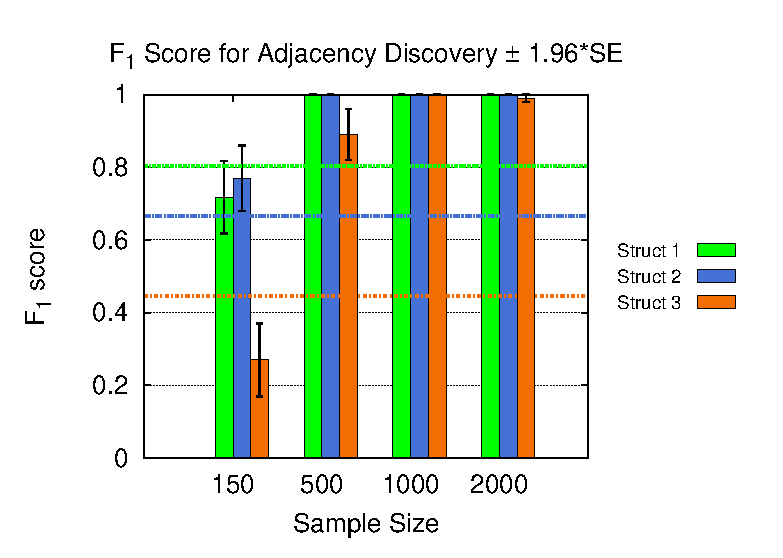
\includegraphics[width=1.1\linewidth]{figures/F1A_single.eps} &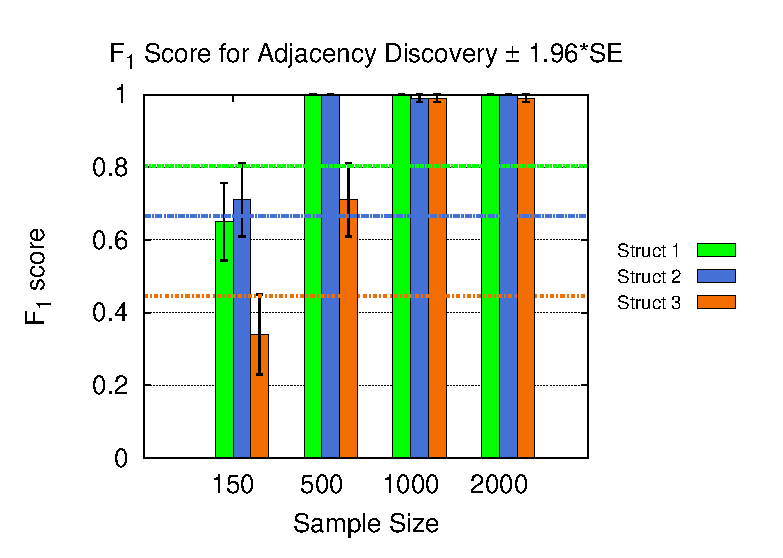
\includegraphics[width=1.1\linewidth]{figures/F1A_multi.eps}\\
				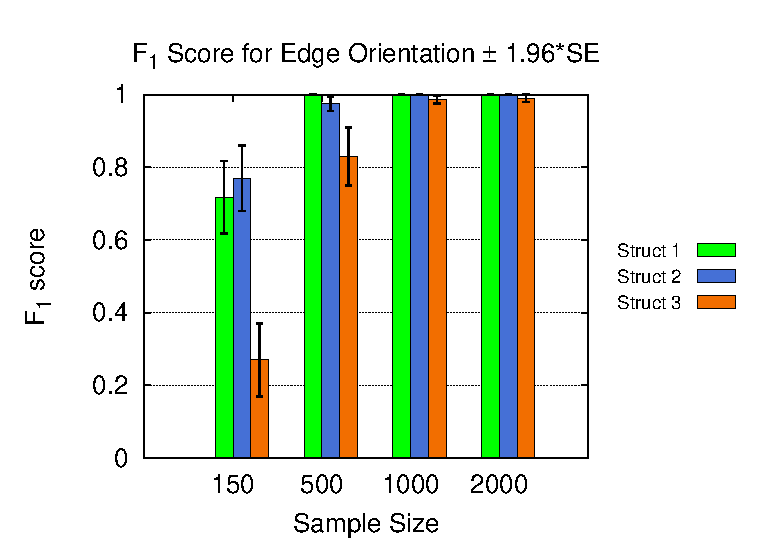
\includegraphics[width=1.1\linewidth]{figures/F1O_single.eps} &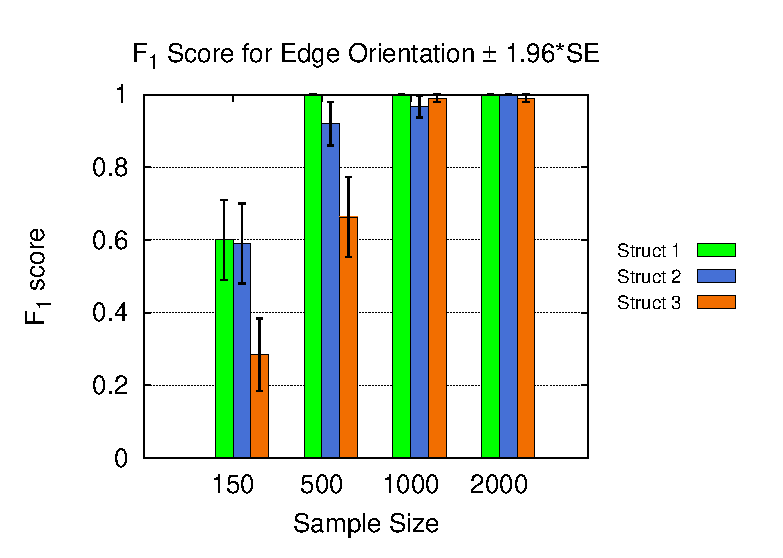
\includegraphics[width=1.1\linewidth]{figures/F1O_multi.eps}\\
				Single Skill& Multiple Skill
			\end{tabular}
		\end{center}
		%\vspace{-0.5em}
		\caption{Comparison of $F_1$ scores for adjacency discovery (top row) and for edge orientation (bottom row). 
			Horizontal lines are baseline $F_1$ scores computed for fully connected (complete) Bayesian networks.} 
		\label{fig:f1-single-multi}
		%\vspace{-1em}
	\end{figure} 
	
	\subsubsection{Sensitivity to Noise}
	
	%\hl{Hard to read}
	Real-world data sets often contain various types of noise.
	For example,  noise may occur due to hidden variables that are not explicitly modeled. 
	%For example, students' performances in a test also depends on their individual ability (in addition to their mastery status of the required skills). 
	%This will create noises in the data if we don't directly model the student's ability.
	To evaluate the sensitivity of REMIND to noise, we synthesize Bayesian networks including a  \emph{StudentAbility} node that takes three possible states (low/med/high). 
	In these Bayesian networks, students' performance depends not only on whether they have mastered the skill, but also on their individual ability. % (in addition to their mastery status of the required skills).
	For simplicity, all items in the setting are single-skilled items. 
	We first simulated data from  Bayesian networks that have a  \emph{StudentAbility} variable to generate ``noisy" data samples, and 
	%There is an arc from \emph{StudentAbility} to each item variable in these data generating models. 
	then use this data to recover the prerequisite structure. % from these truncated data samples. 
	Figure~\ref{fig:stuabilitymodel} illustrates the procedure of this sensitivity analysis experiment.
	
	Figure~\ref{fig:f1-noisy} compare the results were noise was introduced or not.
	Interestingly, the noise does not harm the learning accuracy at all, and actually improves the accuracy.
	We hypothesize that the existence of additional hidden variable increases the variance of the data which can help the structure learning.
	%remove noise by separating students by ability
	%\hl{Can you show the ``true" Bayes net (i.e, with student ability node) and the one we are trying to learn?}
	
	\begin{figure}[!ht]
		\begin{center}
			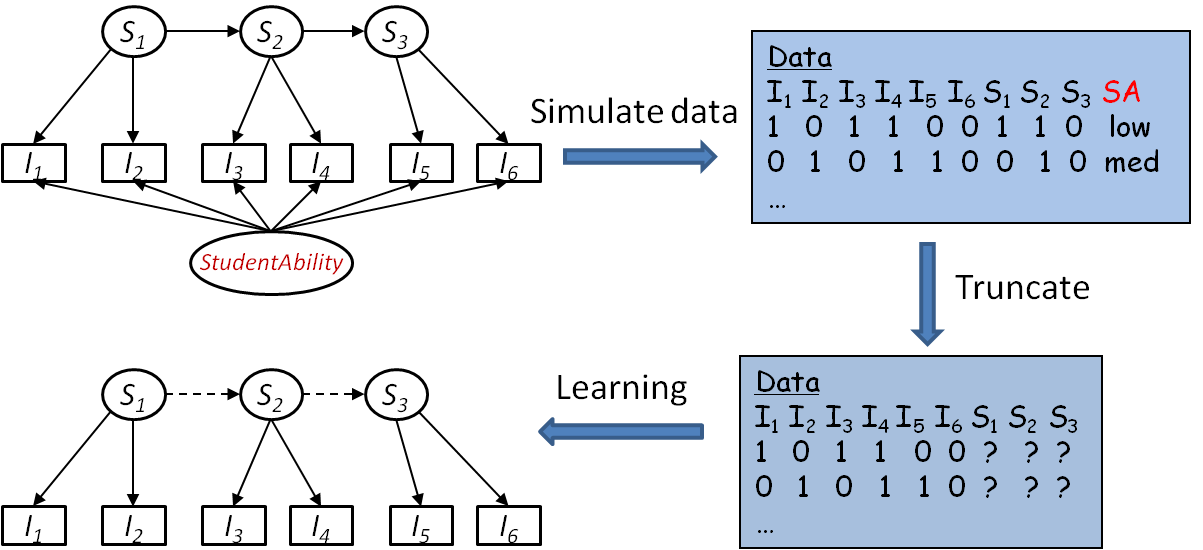
\includegraphics[width=1.0\linewidth]{figures/studentability.png}
		\end{center}
		\caption{Evaluation of BNPD with noisy data} 
		\label{fig:stuabilitymodel}
	\end{figure}
	
	\begin{figure}[!ht]
		\begin{center}
			\centering
			\begin{tabular}{>{\centering}m{1.5in} >{\centering\arraybackslash}m{1.5in}}
				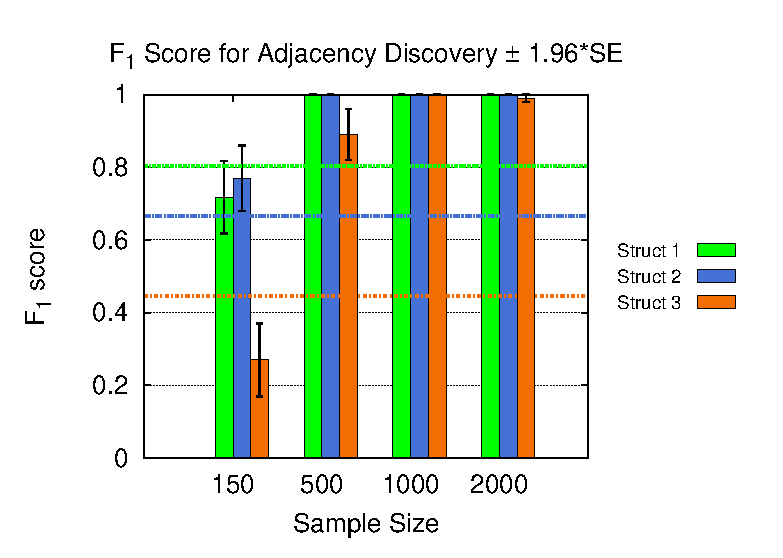
\includegraphics[width=1.1\linewidth]{figures/F1A_single.eps} &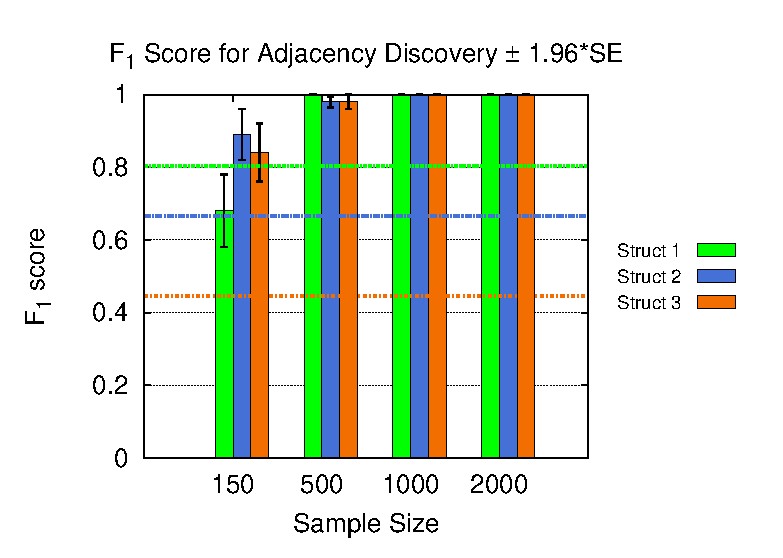
\includegraphics[width=1.1\linewidth]{figures/F1A_single_noisy.eps}\\
				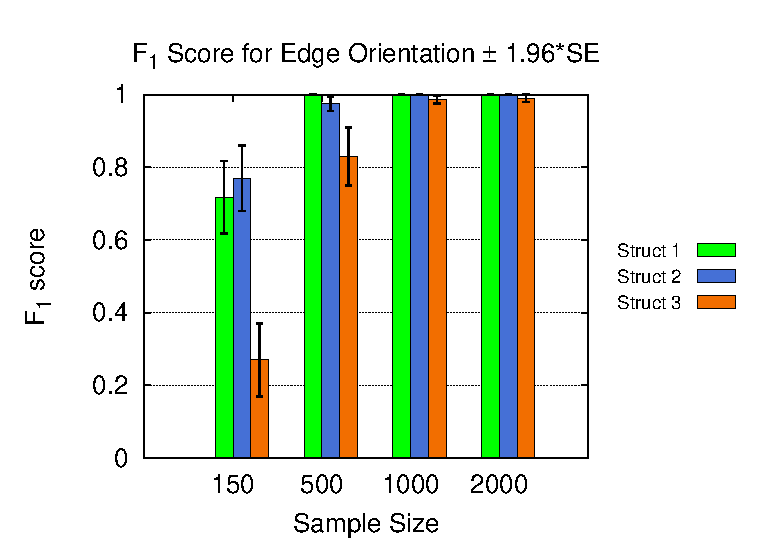
\includegraphics[width=1.1\linewidth]{figures/F1O_single.eps} &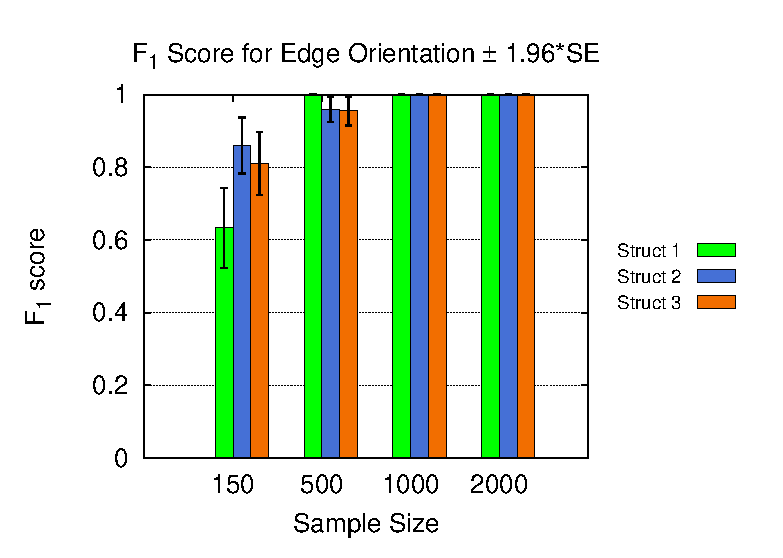
\includegraphics[width=1.1\linewidth]{figures/F1O_single_noisy.eps}\\
				No Noise & Noisy
			\end{tabular}
		\end{center}
		\caption{Results of adding systematic noise. Top: Comparison of $F_1$ scores for adjacency discovery. Horizontal lines are baseline $F_1$ scores computed for fully connected Bayesian networks. Bottom: Comparison of $F_1$ scores for edge orientation. }
		\label{fig:f1-noisy} 
	\end{figure}
	
			\begin{figure}[!ht]
				\begin{center}
					\centering
					\begin{tabular}{>{\centering}m{1.5in} >{\centering\arraybackslash}m{1.5in}}
						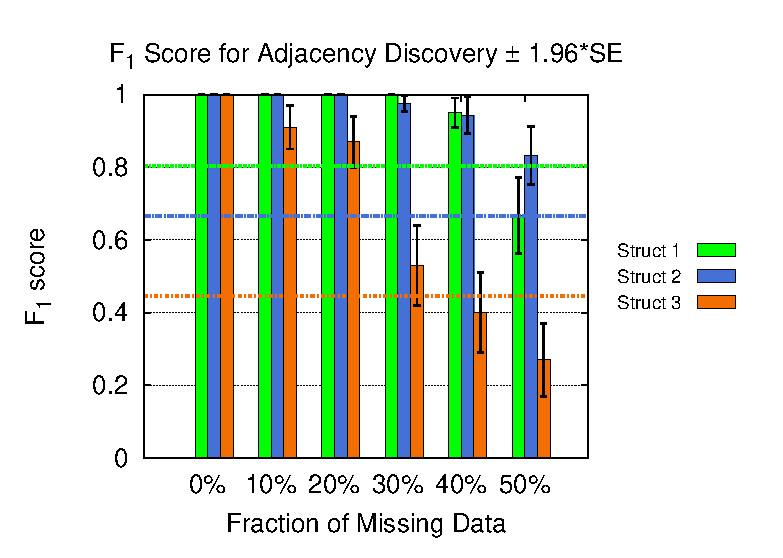
\includegraphics[width=1.1\linewidth]{figures/F1A_single_missing.eps} &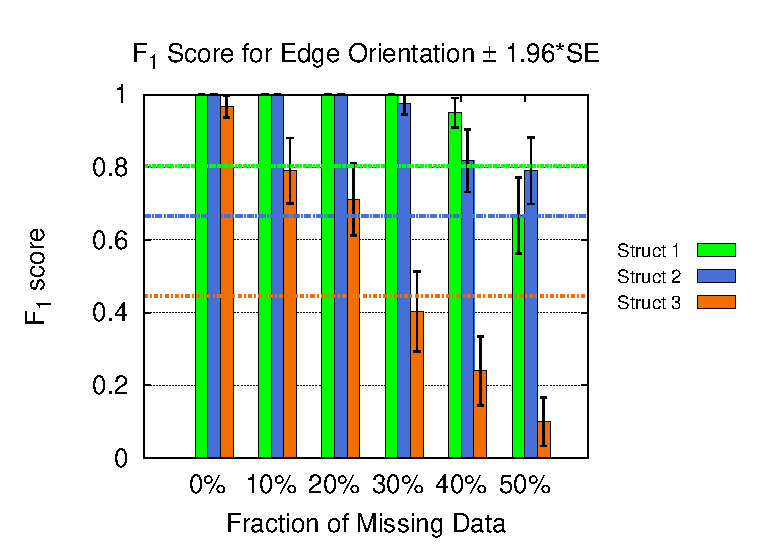
\includegraphics[width=1.1\linewidth]{figures/F1O_single_missing.eps}\\
					\end{tabular}
				\end{center}
				\caption{Results of learning with missing data. Left: Comparison of $F_1$ scores for adjacency discovery. Horizontal lines are baseline $F_1$ scores computed for fully connected Bayesian networks. Right: Comparison of $F_1$ scores for edge orientation. }
				\label{fig:f1-missing} 
			\end{figure} 
	
	\subsubsection{In Presence of Missing Values}
	%Real-world student performance data often has missing data, i.e., some students do not respond to all test items. Structural EM can also be applied with the missing data. 
	%The general idea is, in the E-step, in addition to completing the values for hidden skill variables, the algorithm has to complete the missing data points.
	To evaluate how BNPD performs on data with missing values, we generated data sets of size 1000 with varying fraction of missing values ($10\%$, $20\%$, $30\%$, $40\%$, $50\%$) and ran BNPD to recover the structures from these data sets. Again, the models only contains single-skilled items.  The results are presented in Figure~\ref{fig:f1-missing}.
	It is clearly seen that the accuracy decreases when the fraction of missing values increases. 
	The algorithm is still able to recover the true structures of Structure 1 and 2 even the data contains up to $30\%$ missing values. 
	
	\subsubsection{Comparison With PARM}
	Chen and his colleagues proposed to use Probabilistic Association Rules Mining (PARM) for discovering the prerequisite relationships between skills \cite{chen2015discovering}.
	Since PARM discovers pair-wise prerequisite relationship, instead of constructing the full structure,
	we only compare BNPD with PARM for discovering the pair-wise relationships.
	That is, we derived pair-wise prerequisite relationships from the Bayesian network structure and see how the two approaches discover these relationships.
	Here we simulated data from Structure 3 (Figure~\ref{fig:syn-nets}(c)) (with single-skilled items), which has 21 pair-wise prerequisite relationships.
	When experimenting with PARM, the following cutoff values were used: $ minsup=0.125$, $minconf=0.76$, $minprob=0.9$. 
	These values have been used in the simulation experiments in \cite{chen2015discovering}.
	The evaluation metric used is $F_1=\frac{2*TPR*TDR}{TPR+TDR}$, where $TPR=\frac{\text{\# of correct relationships learned}}{\text{\# of relationships in true model}}$
	and $TDR=\frac{\text{\# of correct relationships learned}}{\text{\# of relationships in learned model}}$.
	The result is presented in Figure~\ref{fig:f1-parm}. It shows that BNPD significantly outperforms PARM $F_1$ score for sample size $n\ge 500$.
	The lower $F_1$ score by PARM is caused by lower $TPR$, i.e., PARM failed to discover many prerequisite relationships (data not shown).
	
		\begin{figure}[!th]
			\begin{center}
				\centering
					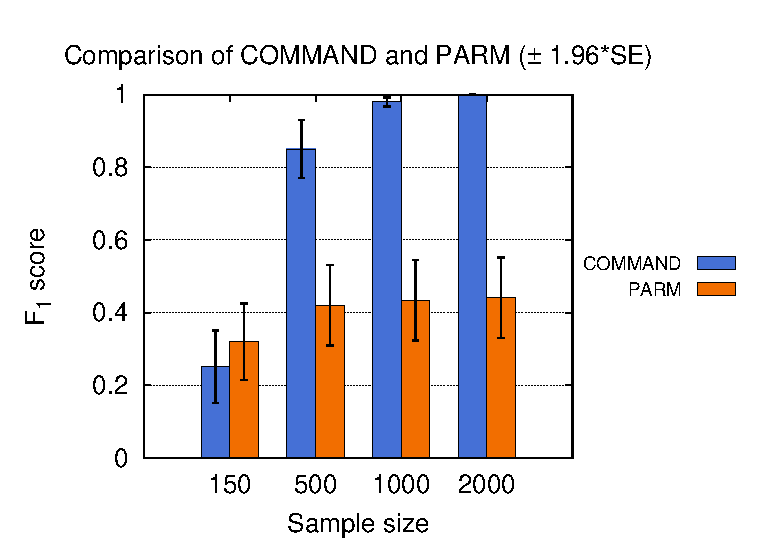
\includegraphics[width=0.7\linewidth]{figures/F1_parm.eps}
			\end{center}
			\caption{Comparison of BNPD and PARM for discovering prerequisite relationships in Structure 3. The cutoff values used for PARM experiments are: $ minsup=0.125$, $minconf=0.76$, $minprob=0.9$.}
			\label{fig:f1-parm} 
		\end{figure}	 
	
	\subsection{Real Student Performance Data}
	\label{sec:real}
	We now evaluate BNPD using two real-world student data sets.
	
	\subsubsection{ECPE Data Set}
	The ECPE (Examination for the Certification of Proficiency in English) data set was collected from a test by the English language Institute
	of the University of Michigan to examine individual cognitive skills required for understanding English language grammar \cite{templin2014hierarchical}.
	It contains a sample of 2922 examinees who is tested by 28 items on 3 skills, i.e., \emph{morphosyntactic rules} ($S_1$), \emph{cohesive rules} ($S_2$) 
	and \emph{lexical rules} ($S_3$). Each item requires either one or two of the three skills. 
	The prerequisite structure output from BNPD are depicted in Figure~\ref{fig:ecpe-result}. The estimated conditional probability tables (CPT) are showed correspondingly.
	The discovered structure says \emph{lexical rules} is a prerequisite of \emph{cohesive rules} and \emph{morphosyntactic rules}, 
	and \emph{cohesive rules} is a prerequisite of \emph{morphosyntactic rules}. 
	This totally agrees with the findings in \cite{templin2014hierarchical} and by the PARM method in \cite{chen2015discovering}.
	%Note that PARM discovered the three pairwise prerequisite relationships but BNPD output a full structure.
	Further, BNPD also outputs the conditional probabilities associated with each skill and its direct prerequisite.
%	which provides insights into how prerequisites impact the post-requisite probabilistically. 
	And we clearly see that the probability of student mastering a skill increases when the student has acquired more prerequisites of the skill.
	
			\begin{figure}[!th]
				\begin{center}
					\centering
					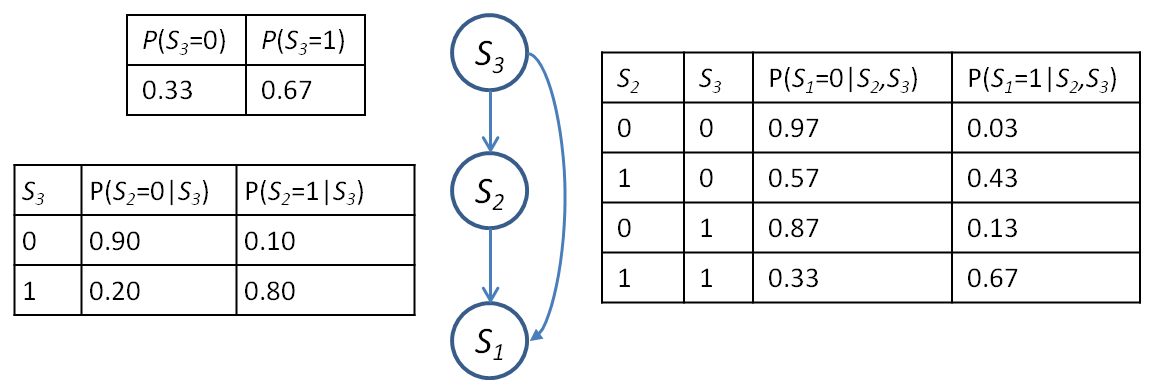
\includegraphics[width=1.0\linewidth]{figures/ecpe_results.png}
				\end{center}
				\caption{Result on ECPE data set. $S_1$: Morphosyntactic rules; $S_2$: Cohesive rules; $S_3$: Lexical rules. 
					The estimated conditional probability tables (CPTs) are shown correspondingly.}
				\label{fig:ecpe-result} 
			\end{figure}
	
	\subsubsection{HED Data Set}
	We now evaluate BNPD using data collected from a commercial non-adaptive tutoring system.
	The data set, named as \texttt{HED}, is from anonymized students interacting with an implementation of a seventh grade math curriculum.
	%This implementation is used by schools (we call it \texttt{traditional}),
	The textbook items are classified in chapters, sections, and objectives; but for this paper, we only use the data from Chapter 2 and Chapter 3 of the book.
	We use performance data while students solve test items.
%	We model the test and homework data using assessment models (\S~\ref{sec:assessment_results}) and learning methods~(\S~\ref{sec:learning_results}), respectively.
	%\texttt{traditional} is much larger data set than \texttt{virtual}.
	%In our experiments, the performance results were converted to binary, i.e., correct or incorrect.
	
	%We first describe our datasets in more detail (\S~\ref{sec:dataset}).
	%We then describe the learned prerequisite structure (\S~\ref{sec:prerequisite_results})
	%as well as our assessment (\S~\ref{sec:assesment_results}) and learning experiments (\S~\ref{sec:learning_results}).
	%In the following assessments, we will use testing results for evaluating the static Bayesian network model and homework for evaluating the PFA models.
	
	%\hl{Mind the note:}
	%Describe digits and connections dataset, without calling them by that names.
	%Call them something else, like "Traditional digital tutor", "Cyber-chart digital tutor"
	%Provide descriptive statistics.
	%Notice that my experiments I use the homework table.  Describe that there are homeworks \& Test
	
	\paragraph{$Q$-matrix and preprocessing}
	\label{sec:preprocessing}
	We use an item-to-skill mapping ($Q$-matrix) that assigns each exercise to a skill solely as the book section in which the item appears.
	%This $Q$-matrix does not convey any information on how or when to offer a remedial intervention to a learner.
	%For this, we investigate the extent on which REMIND can discover a remediation model using student performance data.
	For each chapter, We process the data set to find a subset of  items and students that does not have missing data.
	This is,  the dataset we use in BNPD has students responding to \textit{all} of the  items.
	
	%Table~\ref{tab:seclistdata} lists the twelve skills (book sections) remaining after filtering.
	After filtering, we obtained two data sets, \texttt{HED-chap2} and \texttt{HED-chap3} for Chapter 2 and 3 respectively.  
	In \texttt{HED-chap2}, six skills (book sections) are included and each skill has three to eight items, for a total of 30  items.
	In \texttt{HED-chap3}, seven skills are included and each skill has three to seven items, for a total of 33 items.
	\texttt{HED-chap2} includes student test results for 1720 students;
	while the \texttt{HED-chap3} has the test results for 1245 students.
	%Our synthetic data experiments suggest that a large number of training data improves the learning quality of the prerequisite structure.
	%For this reason, we use the larger \texttt{traditional} dataset to build the prerequisite model.
	
	For simplicity we use binary variables to encode  performance data (i.e, correct or incorrect) and skill variables  (i.e., mastery or not mastery).
	This simplification is not necessary,  as BNPD is able to use  discrete variables with arbitrary number of states.
	
	\paragraph{Prerequisite Structure Discovery}
	\label{sec:prerequisite_results}
	
%			\begin{figure*}[!th]
%				\begin{center}
%					\centering
%					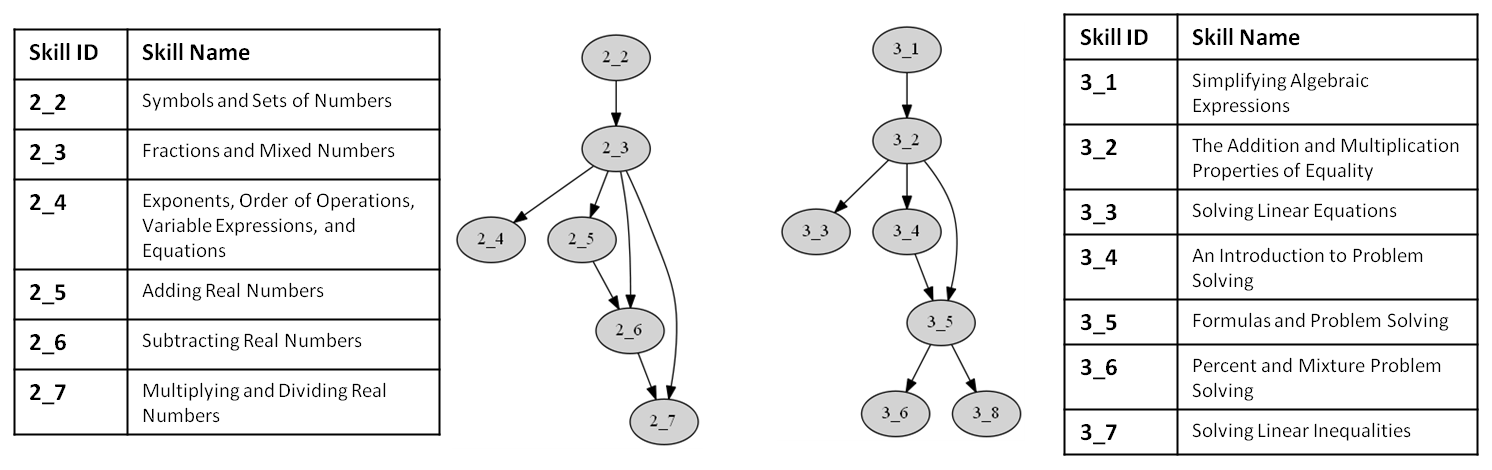
\includegraphics[width=1.0\linewidth]{figures/hed_structures.png}
%				\end{center}
%				\caption{Prerequisite structures constructed by BNPD.}
%				\label{fig:hed-structures} 
%			\end{figure*}

	\begin{figure*}%[ht]
		\centering
		\begin{subfigure}[b]{0.45\linewidth}
			\centering
			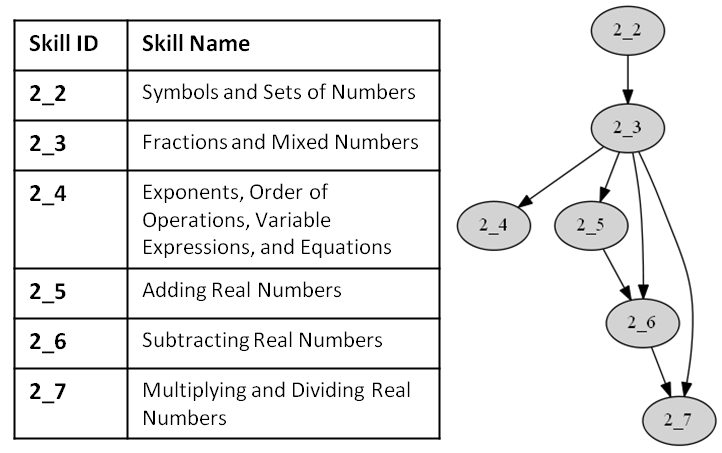
\includegraphics[width=1.0\linewidth]{figures/hed_chap2_structure_prob.png}
			\caption{Prerequisite structure learned for \texttt{HED-chap2}.}
			\label{fig:hed_chap2_structure}
		\end{subfigure}~~~~
		\begin{subfigure}[b]{0.45\linewidth}
			\centering
			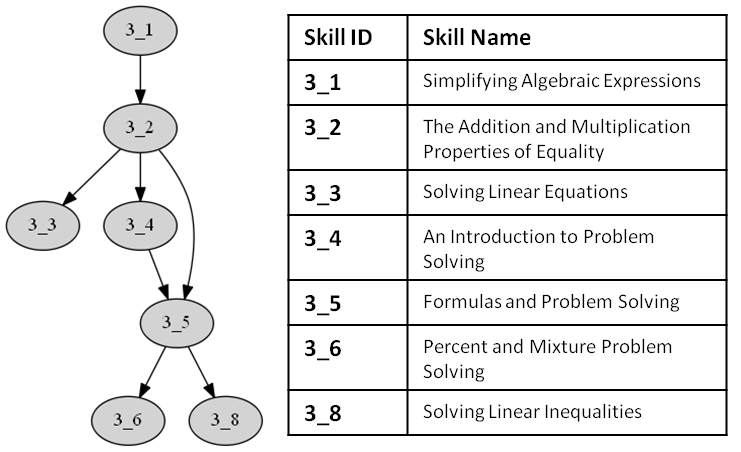
\includegraphics[width=1.0\linewidth]{figures/hed_chap3_structure_prob.png}
			\caption{Prerequisite structure learned for \texttt{HED-chap3}.}
			\label{fig:hed_chap3_structure}
		\end{subfigure}%
		\caption{Prerequisite structures constructed by BNPD for HED data sets.}
		\label{fig:hed-structures} 
	\end{figure*}			
	
	The Bayesian networks generated with the BNPD algorithm are illustrated in Figure~\ref{fig:hed-structures}.
	%Figure~\ref{fig:qmatrix} represents a disconnected model generated by simply converting the input $Q$-matrix into a Bayesian network;
	%this corresponds to the output of the initialization step of Algorithm~\ref{alg:remind}.
	%Figures~\ref{fig:constraint} and~\ref{fig:noconstraint} represent the prerequisite structures discovered by using domain knowledge or not.
	%In the fully data-driven model, we draw with red the edges that contradict our text book ordering heuristic.
	%Note that some edges are undirected indicating these directionalities of these edges can not determined given the observational data.
	%Our observation is that the structures learned are not random, sections (skills) in the same chapter tend to form clusters, 
	%even in the structure learned without the ordering constraint.
	Our observation is that the topological order of the sections in both structures are fully consistent with the book ordering heuristic,
	This shows an agreement between our fully data-driven method and human experts.
	We also ran PARM approach to learn pair-wise prerequisite relationships from these data sets.
	For \texttt{HED-chap2}, PARM outputs two relations: $2\_5\rightarrow 2\_6$ and $2\_5\rightarrow 2\_7$  
	%The inferred prerequisite structures are intuitively plausible, 
	%as the topological order of the sections are consistent with the book structure, which reflects subject matter experts's belief on the prerequisite relationships 
	%between the sections of each book chapter. 

%	Our approach also outputs the conditional probabilities associated with each skill and its direct prerequisites.
%	Figure~\ref{fig:chap123noorderCPT} plots the conditional distribution table for each skill.
%	Each sub-figure plots the conditional probability of student achieving the mastery of a skill against the mastery status of the skill's direct prerequisites. 
%	More specifically, X-axis specifies all possible mastery statuses of a skill's direct prerequisite, 
%	Y-axis is the probability of student achieving the mastery of the skill given the corresponding mastery status of its direct prerequisites.
%	We can see a trend in all plots that the probability of student mastering a skill increases monotonically when the student has acquired more prerequisites of the skill.
%	This is consistent with our intuition that mastering a skill's prerequisites will help student master the skill.
%	We also observed a small contradiction in the case of skill 3-2, which exemplifies the limitation of fully data-driven methods. 
	%\hl{Please describe this figure with much more detail than this.  This currently does not have enough explanation to be understandable}
	
	\paragraph{Predictive Performance of Prerequisite Models}
	\label{sec:predictive_performance}
	BNPD not only discovers the topological relationships among skills, but also outputs a statistical model in the form of Bayesian network.
	This statistical model can be used for inference and predictive modeling. 
	%We now evaluate  REMIND using data  that has already been collected (\textit{post-hoc} analysis). %an evaluation of the REMIND algorithm using  . 
	We now evaluate how well the generated Bayesian networks can predict student performance
	%student's knowledge about a skill given his/her performance on any of the test items. 
	%Since student's knowledge about a skill is not directly observed, 
	%we are unable to assess the predictive performance of these models involved in this task.
	%However, we have direct observations on students' performance on test items. 
	%For this, we evaluate  predicting student performance
	on a test item given performance on other items.
	In particular, we compute the posterior probability of a student's response to an item $I_i$ given his performance on all other items 
	$\mathbf{I}_{-i}=\mathbf{I}\setminus\{I_i\}$, by marginalizing:
	\begin{align}
		P(I_i=1|\mathbf{I}_{-i}=\mathbf{i}_{-i}) =\sum_{\mathbf{S}}P(I_i, \mathbf{S}|\mathbf{I}_{-i}=\mathbf{i}_{-i}),
	\end{align}
	This can be computed efficiently using the Junction tree algorithm \cite{koller2009probabilistic}. 
	We then do binary classification based on the posterior probability.
	
	We compare the Bayesian network models generated from BNPD with four baseline predictors:
	\begin{itemize}
		\item  A \emph{majority} classifier which always classifies  an instance to the majority class.
		For example, if majority of the students get an item wrong, other students would likely get it wrong.
		\item  A Bayesian network model in which the skill variables are \emph{disconnected}. 
		This corresponds to using the $Q$-matrix  Bayesian network of Figure~\ref{fig:qmatrix}.
		This model assumes that the skill variables are marginally independent of each other.
		\item A Bayesian network model in which the skill variables are connected in a \emph{chain} structure, i.e., 2-2$\rightarrow$2-3$\rightarrow$2-4$\rightarrow\dots$
		This assumes that a section (skill) only depends on the previous section.
		In other words, a first-order Markov chain dependency structure.
		\item A \emph{fully connected} Bayesian network where skill variables are fully connected with each other.
		This model assumes no conditional independence between skill variables and can encode any joint distribution over the skill variables.
		However, it has exponential number of free parameters and thus can easily overfit the data.
	\end{itemize}

	\begin{figure}[!ht]
		\centering
		\begin{subfigure}[b]{1.0\linewidth}
			\centering
			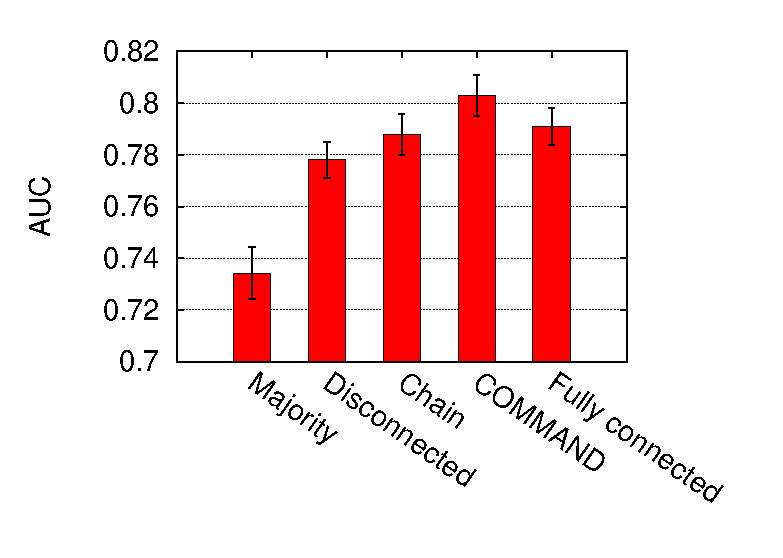
\includegraphics[width=0.8\linewidth]{figures/hed_chap2_30_auc.eps}
			\caption{\texttt{HED-chap2} AUC results. }
			\label{fig:auc-chap2}
		\end{subfigure}\\
		\begin{subfigure}[b]{1.0\linewidth}
			\centering
			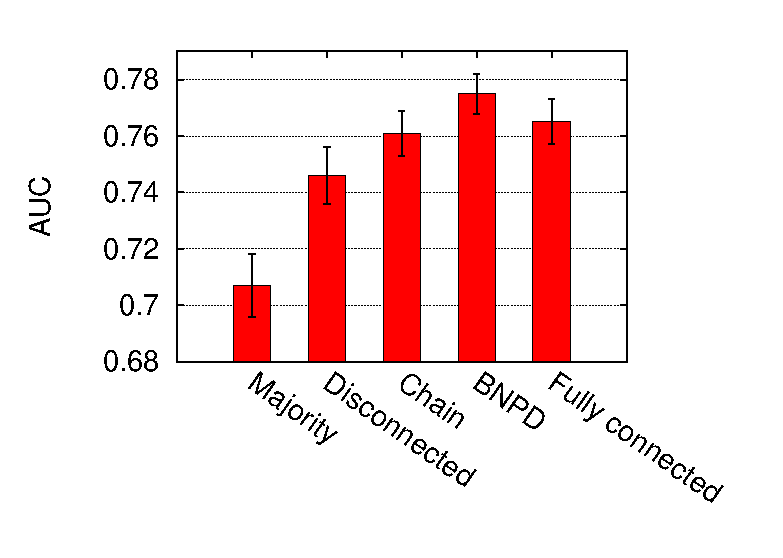
\includegraphics[width=0.8\linewidth]{figures/hed_chap3_33_auc.eps}
			\caption{\texttt{HED-chap3} AUC results.}
			\label{fig:auc-chap3}
		\end{subfigure}%
		\caption{Comparison of AUC of five models to predict student performance on test items. The results are from 10 fold cross-validation.\label{fig:aucs}}
	\end{figure} 	
	
	The parameters of these baseline Bayesian network predictors are estimated from the data.
	We did 10-fold cross-validation to evaluate the classifiers.
	The model predictions were evaluated using the \textit{Area Under the Curve} (AUC) of the Receiver Operating Characteristic (ROC) curve metric.
	Results are presented in Figure~\ref{fig:aucs}. 
	The error bars show the $95\%$ confidence intervals calculated from the cross-validation.
	For both \texttt{HED-chap2} and \texttt{HED-chap3} data sets, the best performing models are BNPD models, with an AUC of $0.803\pm0.008$ (Figure~\ref{fig:auc-chap2}) and an AUC of $0.775\pm0.007$ (Figure~\ref{fig:auc-chap2}), respectively. % and correspond to and no constraints, respectively.
	%these models are: $0.691\pm0.011$ (\emph{majority}), $0.761\pm0.007$ (\emph{disconnected}), $0.796\pm0.006$ (\emph{chain}),  $0.804\pm0.007$ (\emph{prerequisite model with order constraint}), $0.807\pm0.006$ (\emph{prerequisite model without order constraint}), $0.794\pm0.007$ (\emph{fully connected}).
	%The comparison of the Area Under Curve (AUC) \todo{Area of what curve? ;-)} for these classifiers is presented in Figure~\ref{fig:auc-cv}.
	%These two REMIND models outperform the other four models.
	%\hl{How much is the AUC, though? Explain the graph with words here}
	The \emph{fully connected} model performs the best among the four baseline predictors with an AUC of $0.796\pm0.006$.
	A paired $t$-test reveals that both of the REMIND models significantly outperform the \emph{chain} model (the $p$-values are 0.0064 and 0.003).
	However, the two REMIND prerequisite models are not statistically different from each other. 
	We note that the \emph{fully connected} model was outperformed by the two prerequisite models and the \emph{chain} model, suggesting  overfitting.% might have happened. 

	
	\section{Conclusion and Discussion \label{sec:conclusion}}
	We believe we are the first ones to propose a pipeline of learning the prerequisite dependencies from data and use it for student modeling. 
	Our work builds on prior work that discovers prerequisite  from data \cite{desmarais2006learned,vuong2010method, brunskill2010estimating,scheines2014discovering,chen2015discovering,piech2015deep}.
	However, these approaches do not attempt to validate the prerequisite discovered using real student performance data.
	Our approach differs from prior work in several ways.
	The approaches  discover the relationship of items without using latent variables.
	This is, the prerequisites do not use skill mappings, and only find dependencies between items~\cite{desmarais2006learned,vuong2010method,piech2015deep}.
	%i.e., the item-level prerequisite relationships, while we try to discover the prerequisite relationships between hidden skills.
	For the approaches that can account for latent variables~\cite{brunskill2010estimating,chen2015discovering}, they focus on estimating the pairwise prerequisite relationships.
	By contrast, we try to optimize the full structure of the model.
	
	A contribution of our work is introducing the Structural EM algorithm to the educational community.
	This approach has many advantages over prior work in that it does not require tuning of many parameters.
	For example, prior work~\cite{brunskill2010estimating} assumes  domain parameters called \emph{guess probability} and \emph{slip probability}
	%\footnote{The \emph{guess probability} is the probability of answering the correctly given the student does not know the skill; the \emph{slip probability} is the probability of answering incorrectly given the student knows the skill} 
	are provided for each pair of item and skill.
	Similarly, more recent approaches~\cite{chen2015discovering} require manually specified thresholds to determine the existence of a prerequisite relationship.
	The determination of these thresholds requires experts' intervention. 
	By contrast, the only required input of our algorithm is the observed student performance.
	
	%\hl{Two parts: Prerequisite discovery and student modeling with multiple kcs}
	%\hl{For prereq work: Cite Ilya's work, French lab, Thorsten's work, may be Deep KT work}
	%\hl{Have a comparative table of prereq work}
	%\hl{For student modeling with multiple KCs cite LR-DBN work by YanBo, Topical HMM \&FAST work by Jose, conjunctive kt by Ken Koedinger}
	
	\section{Conclusion}
	Although in some educational paradigms~\cite{koedinger2010knowledge} students are not supposed to move to subsequent lessons until they have mastered all of the prerequisites, these is not always attainable in practice.
	We propose and evaluate the REMIND pipeline, a simple but effective novel algorithm that detects when a student needs remediation.
	
	A limitation of our study is that we only evaluated REMIND using simulations and posthoc analyses.
	Future work may evaluate the REMIND algorithm in a randomized control trial.
	Further, we evaluated our models using traditional statistical metrics, 
	but recent work suggest that tailored evaluation metrics for tutoring system may be superior \cite{leopard_edm}.
	Thus, another piece of future work is to evaluate REMIND using these evaluation metrics.
	
	The main contributions of our work are:
	a novel data-driven algorithm that allows domain knowledge for designing remediation triggers;
	a novel methodology to evaluate prerequisite graphs using student data;
	and suggesting the Structural EM algorithm for educational applications.
	
	The advantage of REMIND are both qualitative and quantitative.
	Qualitatively, REMIND allows us to understand the organization of the skills in the curriculum as it builds a prerequisite network of the skills in a $Q$-matrix.
	When used in a learning model, REMIND builds a hypothesis of how practice affects the knowledge of the student.
	Sometimes the practice may affect the skill directly, but sometimes it may affect a prerequisite.
	Future work may validate these hypothesis in a controlled experiment.
	Additionally, our quantitative results suggest that REMIND can be used to improved student modeling.
	Overall, we believe that REMIND is promising technology to detect when a student needs help.
	
% REFERENCES FORMAT
% References must be the same font size as other body text.
\bibliographystyle{SIGCHI-Reference-Format}
{%\small
	\bibliography{references}
}	

\end{document}
